\section{Constraint Motif Mining and EGH for Prediction}
Modeling activity of daily life (ADL) has become a burgeoning research topic, 
since people demand a comfortable life at home
at a lower cost. 
Since heating and cooling spaces consumes $\sim$53\% of the total electrical usage 
by heating and cooling spaces %\cite{energydatabook2011} 
of an average household, 
automating the operation of HVAC devices to save energy is important. 
One of the crucial components required to achieve this goal is 
to model and predict the occupancy of a home. 
Supervised learning approaches on the analysis of indoor temperature~\cite{kleiminger2014predicting}, 
smart phones' GPS data~\cite{koehler2013therml}, 
electricity consumption~\cite{erickson2010occupancy} and 
sensor data by tracking indoor activities~\cite{scott2011preheat,alrazgan2011learning} 
are effective ways to approach this prediction problem. 
Prediction of occupancy using sensor data has been broadly researched. 
By capturing daily activities, like room occupancy of the house, 
usage of electrical devices, 
and usage of water systems using sensors, 
researchers have modeled occupancy~\cite{mahmoud2013behavioural,erickson2010occupancy,beltran2014optimal} 
and used these results to automate the control of the HVAC system. 

Although the supervised learning kNN~\cite{scott2011preheat}, 
neural network~\cite{mahmoud2013behavioural} and Markov model~\cite{erickson2010occupancy} 
are effective, 
the detailed household activities represented as a time series are not fully utilized. 
Daily activities such as waking up, cooking, washing, and commuting to work/school and back 
have different patterns based on the day. 
For instance, the schedule on a working day is significantly different from that of a weekend 
or a holiday. 
Thus, this scenario leads itself to episode mining analysis, 
which can be used to predict household occupancy. 
Using this strategy of episode mining for occupancy prediction has three advantages. 
First, episode mining, a temporal mining approach, mines according to the time 
distribution for each type of activity. 
Second, it builds the activity scenario and connects the episode with 
a probabilistic hidden Markov model (HMM). 
Unlike previous models, 
the time and order of each kind of activity are fully utilized. 
Third, the algorithm predicts according to the scenario-based probabilistic model episode 
generative HMM (EGH). The prediction accuracy is better than the existing models. 

%This work's contributions can be highlighted in the form of the three questions below. 
%\begin{enumerate}
%\item How can we mine for meaningful scenarios? 
%Episode mining can mine many frequent episodes, but not all the episodes are useful 
%for occupancy prediction. 
%By narrowing the episodes according to the start state, 
%end time, event dwelling time and the gap between two activities, 
%we can interpret these episodes and provide insight as to 
%which episodes are informative. 
%\item How can we predict the occupancy more accurately?
%Our dataset comprises detailed information of the various activities of a household 
%tracked as a time series on a daily basis. 
%Thus our episodes have rich detailed information based on occupancy and 
%unoccupancy of the household. 
%Since we are mining episodes from this data, 
%the accuracy of occupancy prediction improves significantly. 
%\item  Can it help save electric usage at home?
%The prediction occurs at least 15 minutes ahead of a person 
%leaving or coming back. 
%By connecting this prediction result to an automatic HVAC controlling system, the HVAC can be turned on or off  ahead of the occupancy change. 
%Since the HVAC does not work during occupancy, 
%this saves electric usage. 
%\end{enumerate}

\subsection{Occupancy Prediction Problem Formulation}
Given $M$ time series, 
each time series $X^{(m)}=X^{(m)}_1, ..., X^{(m)}_t, ..., X_T^{(m)}$ 
represents a sequence of room occupancy of person $m$ inside 
a home over $K$ days, 
where $X_t\in s$ denotes that $X$ belongs to a finite room set $s$ at the sequence number of $t$, 
and $m\in\{1,...,M\}$. 
%Each $X$ is has a start time $X.start$ and an end time $X.end$.  
Let $Z$ denote that the home is unoccupied and $Z\in s$.  %$Z=0$ if a house is unoccupied; $Z=1$ if the house is occupied.  
%Its meaning equals to certain symbols from set $s$. 
We predict whether person $m$ stays at home the rest of a day from time $T$,  i.e. during $T+1$, $T+2$, ..., $\Delta T$, 
 
\begin{equation}
\hat{Y}^{(m)}=\hat{Y}_{T+1}^{(m)},...,\hat{Y}^{(m)}_{T+\Delta T}
\end{equation}
where $Y_{T+\Delta t }^{(m)}=Z$ if person $m$ does not stay at home at time $T+\Delta t $;
otherwise, $Y_{T+\Delta t}^{(m)} \neq Z$. 
%The un-occupancy of the whole house is the intersection of un-occupancy of all people. 
If any person $m$ stays at home $Y_{T+\Delta t}^{(m)} \neq Z$, then this house is occupied $Y_{T+ \Delta t} \neq Z$. 


\subsection{Temporal Mining Mixture Model}
We use a three-pronged approach to tackle the problem of mining and predicting unoccupancy, as 
shown in Figure~\ref{fig_framework}.
\begin{figure}[h]
\centering
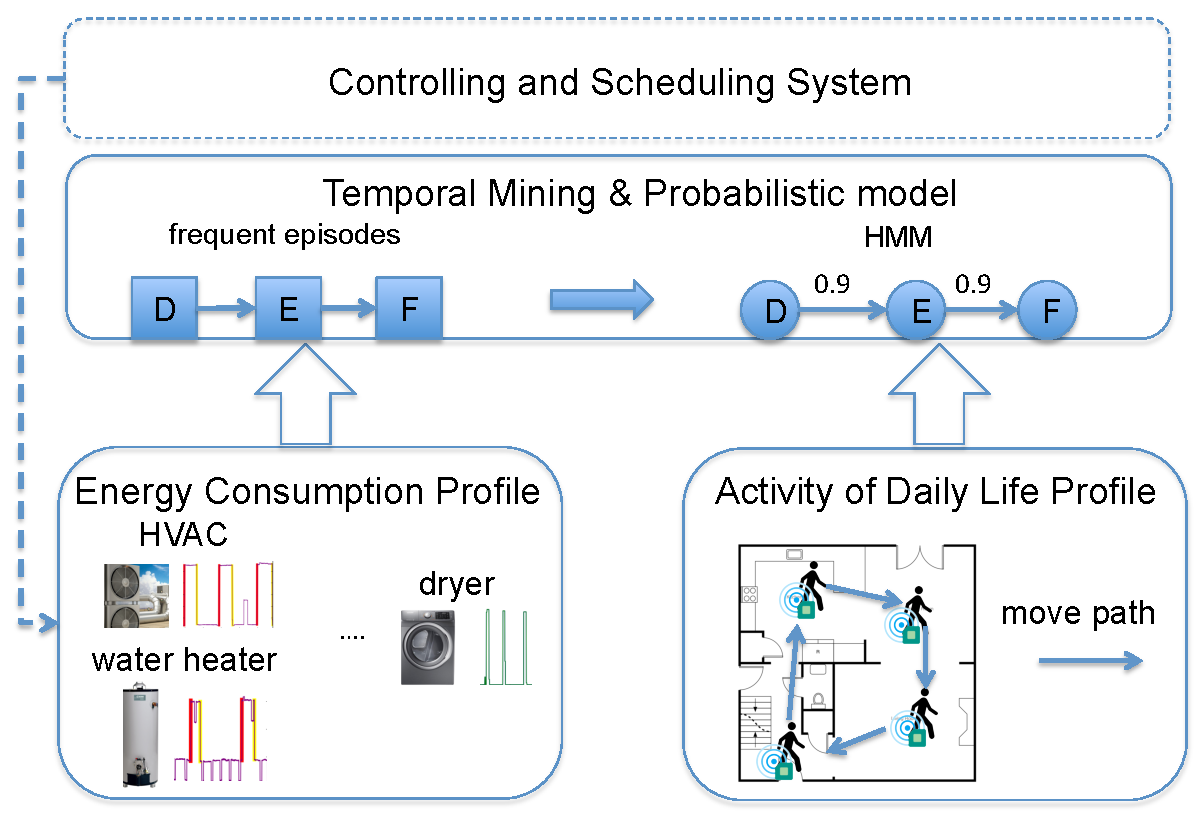
\includegraphics[width=0.5\textwidth]{adlfigs/framework.pdf}
\caption{Occupancy Prediction Framework.\label{fig_framework}}
\end{figure}
Given indoor activities time series of a person over a period of time, 
first, we use an episode mining algorithm to discover frequent episodes from the past days' data. Then we connect each episode with an EGH and build a mixture EGH model. 
Based on the mixture model, we predict when each person will leave and come back the house. 
If all people leave, then the house is unoccupied. 

%Before formalizing the problem statement, we introduce several concepts and notations. 

\textit{Episode} 
An episode is a collection of ordered events. 
Here an episode refers to an ordered events which are 
highly relevant to the occupancy status inside a building. 
For instance, we represent 'S' as sleep, 
'K' as kitchen, and 'Z' as going out. 
If an episode $S \rightarrow K \rightarrow Z$ is found, 
the story is described as a person getting up, 
going to the kitchen for breakfast, and then leaving the house. 
An episode $\alpha$ is composed 
of a series of ordered events
$\alpha=\langle X_1,..,X_t,...X_T \rangle$, 
where $X_t$ denotes that $X$ occurs at a sequence of $t$.  
The event $X_t$ may be the point event or dwelling event. 
The dwelling event
has a start time $X.start$ and end time $X.end$. 
In this paper  $X$ denotes a dwelling event and 
represents which room a person stays 
inside a building, i.e., this building is \emph{occupied}. 
Since $Z$ denotes a room is unoccupied, 
$Z.start$ is the point at which a person or all people inside the building leave, and 
$Z.end$ is the point at which a person or all people come back. 

%\textit{EGH} Episode generative HMM model is a 
%type of HMM model which connects each episode $\alpha$ 
%with a special HMM model $\Lambda_\alpha$. 
%The uniqueness of the EGH is that 
%the transition matrix and 
%emission matrix is only decided by a noise parameter $\eta$. 
%The value of $\eta$ is computed based on the frequency of the 
%corresponding episode $\alpha$. 

\subsection{Time-gap Constraint Episode Mining}
\textbf{Episode Mining}
Episode mining has been studied in previous research \cite{mannila1997discovery}. 
It uses a non-overlap mining approach to find the frequent episodes. 
Episode mining has been applied to energy disaggregation to help conserve energy in buildings~\cite{shao2013temporal} in sustainability research. 
In contrast with previous research, 
the events in this application of occupancy prediction 
dwell at an event for a period of time. 
As a result, we extend the above two 
episode mining algorithms~\cite{laxman2008stream,patnaik2008inferring} 
and enforce more constraints.
One change is to 
adopt right alignment for the first element in the episode mining. 
%In the example of $AB$, 
%the mined second instances is $\langle A_9,B_{11} \rangle$. 
The second modification is to 
add time constraints and 
apply gap duration constraints between 
two consecutive events inside an episode. 
%Figure \ref{fig_durationgapconstraint} shows an example of time-gap constraint episode. 
%\input{adlfigs/durationgapconstraint.tex}
\input{adlfigs/MingExample.tex}
Figure~\ref{fig_MingExample} shows a time-gap constraint episode mining example. 
Let us assume we have a frequent episode $S\rightarrow B \rightarrow K\rightarrow Z$. 
We then add the time constraints to each event $\{S,B,K,Z\}$. 
The dwelling duration of $S$ is 3 to 6 hours,   
of $B$ is 2 to 20 minutes, 
of $K$ is 5 to 60 minutes, 
and of $Z$ is 3-9 hours. 
In addition, we set gap duration between any two consecutive events. 
The gap duration of $SB$ is calculated as $\Delta{SB} = B.start-S.end$. 
We set the maximal gap time between SB, BK, and KZ as 
10 minutes, 40 minutes and 100 minutes; 
the minimal gap time is 0. 
Then we have a stream composed of the sequence of dwelling events "Event seq," as shown 
in Figure~\ref{fig_MingExample}.  
 The time-gap constraint episode mining process 
 to discover a frequent episode uses the following method. 
 Let the $node$ structure denotes each element in any episode,  
as depicted as a square box in Figure~\ref{fig_MingExample}.  
Let $waits$ refer to a structure which pairs with an episode 
and has the same length of this episode. 
Initially, a $waits$ structure related to episode $S\rightarrow B \rightarrow K\rightarrow Z$ is created. 
A $node$ structure related to $S$ is created 
and it waits for the first 
element of the episode $S\langle 180, 360 \rangle $. 
When $T=1$, the duration of $S_1$ is checked. 
Since $S_1$ is in the range of $3-6$ hours, 
$S_1$ passes and is put into the node structure $node$ related to $S$. 
Next a new $node$ structure is created to wait for $B\langle 2, 20 \rangle $. 
When $T=2$ and $T=3$, both $B_2$ and $B_3$ 
are qualified in terms of the time constraints and 
the gap constraints; 
e.g., the gap between $S$ and $B$ $\Delta SB$ should 
be between 0 and 10 minutes. 
These two nodes $B_2$ and $B_3$ are then input into the 
$waits$ structure. 
At the same time, 
a new $node$ structure is created for $K\langle 5, 60 \rangle $. 
When $T=4$, the gap between $\langle B_3, K_4 \rangle$ 
is satisfied with the distance condition between 
$B$ and $K$ 0-40 minutes. 
However, the gap between $\langle B_2, K_4 \rangle$ 
is longer than the constraint gap. 
Therefore, $B_2$ is canceled out. 
Now a new $Z$ waits for the symbol $Z\langle 180, 540 \rangle$. 
When $T=6$, the gap from $B_2$ to $K_6$ is 
too large. Therefore, $K_6$ is not added into the $node$ $K$ structure in $waits$.
When $T=8$, the duration of $Z_8$ does not qualify for the condition of between 3-9 hours,  
so $Z_8$ is not added. 
When $T=10$, the duration of $Z_{10}$ meets the requirement of between 3-9 hours 
and its distance to $K4$ meet the requirement 
of $\Delta KZ \in [0,100]$ minutes. 
Thus $Z_{10}$ is added into the $node$ $Z$ structure in $waits$.
Therefore, complete mining of an episode is complete, and 
we have mined two instances here; $S_1B_3K_4Z_{10}$ and $S_1B_3K_6Z_{10}$. 

%This complete gap-constraint episode mining on dwelling events 
%is described in detail in Algorithm \ref{alg_episodeMiningConstraint}
%\ref{alg_episodeMiningConstraint_2e} 
%in the appendix section.

%Non-overlap episode mining is defined as \textit{Definition}. 
\subsubsection{Mixture EGH}
\textbf{Episode Generating HMM}
Episode generative HMM (EGH) model is a 
type of HMM model which connects with frequent episode, 
and the more frequent an episode inside a sequence, 
the likelihood of the state sequence including this episode is larger~\cite{laxman2008stream}.  
%$\alpha$ with a special HMM model $\Lambda_\alpha$. 
The uniqueness of the EGH is that 
the transition matrix and 
emission matrix is only decided by a noise parameter $\eta$. 
The noise parameter $\eta$ of frequent episode $\alpha$ 
is calculated as $\eta=\frac{T-Nf_{\alpha}}{T}$,  
where $T$ is the training data stream length, 
$\alpha$ is the frequent episode, 
$N$ is the length of frequent episode $\alpha$, 
$f_{\alpha}$ is the frequency over the time $T$.

%% not sure whether should be included 09112015
In the mixture EGH model shown in Figure \ref{fig_egh}, 
the transition matrix of an EGH is given as an example. 
Let us assume we have a N-node frequent episode $S\rightarrow B\rightarrow Z$, where $N=3$.
We define 2N number of hidden states; 
N for episode states, and N for noise states. 
The noise states are $\{W, X, Y\}$. 
An episode state transfers to another episode state 
at the probability of $1-\eta$.
An episode state transfers to a noise state 
at a probability of $\eta$. 
A noise state transfers to another noise state 
at a probability of $1-\eta$. 
To calculate the emission matrix, first we 
let M denote the total number of symbols in the event stream. 
For any hidden states in the episode, M has a delta function emission. 
Whenever it is visited (right alignment of the first element in the episode, 
left alignment for the left elements in the episode), 
it will generate the same observation symbol. 
For any noise hidden states, it emits any of the symbols from the $M$ 
observation symbols with a uniform distribution at probability $\frac{1}{M}$. 
\input{adlfigs/egh.tex}

Theorem \ref{theorem1} from \cite{laxman2008stream} is crucial.  
The theorems in \cite{laxman2008stream}
prove that the more frequent an episode is inside a sequence, 
the greater the likelihood of the state sequence including this episode. 
The proof for this theorem is explained in detail in \cite{laxman2008stream}. 


\newtheorem{mydef}{THEOREM}
\begin{mydef}
\label{theorem1}~\cite{laxman2008stream} 
Let $D_Z={X_1,..., X_K}$ is the given sequence data,  $\varepsilon$ is the symbol set, 
and the size of these symbols is $M$. 
Given two frequent N-node episodes $\alpha$ and $\beta$ with frequency $f_{\alpha}$ 
and $f_{\beta}$. Their corresponding EGH is $\Lambda_{\alpha}$ and $\Lambda_{\beta}$. 
The most likely state sequence for episode $\alpha$ and $\beta$ are
$q_{\alpha}^*$ and $q_{\beta}^*$. 
The noise parameters of these two EGH are 
$\eta_{\alpha}$ and $\eta_{\beta}$. 
Assume both of these noise parameters are less than $\frac{M}{M+1}$, 
we have 
(1) if $f_{\alpha} > f_{\beta}$, then $P(D_Z, q_{\alpha}^*| \Lambda) > P(D_Z, q_{\beta}^*| \Lambda)  $
(2) if $P(D_Z, q_{\alpha}^*| \Lambda) > P(D_Z, q_{\beta}^*| \Lambda)  $, $f_{\alpha} > f_{\beta}$
\end{mydef}

\textbf{Mixture Model}
The mixture EGH model is fully discussed in previous work \cite{laxman2008stream}.
This model 
gives different weights to each EGH
to predict a target event. 
We can assume we obtain whether an episode occurs on a certain day. 
Let $D_Z=\{X_1,..., X_K\}$ denote the $K$ days data set. 
$F=\{\alpha_1, ... \alpha_J\}$ denote the frequent episodes in the dataset $D_Z$. 
An EGH $\Lambda_{\alpha_j}$ 
is associated with frequent episode $\alpha_j$.
$\Lambda_Z$ denotes a mixture EGH model. 
The likelihood of $D_Z$ under the mixture model is written as Equation (\ref{eq_mixture}).
\begin{eqnarray}
\label{eq_mixture}
Pr(\Lambda|Z) &=& \prod_{i=1}^K P[X_i|\Lambda_Z] \\
			&=& \prod_{i=1}^K ( \sum_{j=1}^J \theta_j P[X_i| \Lambda_{\alpha_j}])
\end{eqnarray}
where $\theta_j$ is the mixture coefficient of $\Lambda_{\alpha_j}$ and it subjects to 
$\sum_{j=0}^J \theta_j=1$ 

The parts inside Equation (\ref{eq_mixture}) are additive; 
the coefficients $\theta$ are computed by EM algorithm. 
%The detailed description is algorithm %%%\ref{alg3} 
%in the appendix section.
%\input{adlalgs/alg03.tex}
During the initialization %line 1-10
part of the EM algorithm, 
the episode frequency over the times series T over $K$ days is calculated. 
Specific frequent episodes ended with target event 'Z' are selected. 
Optionally, 
we could add special constraints on episodes, starting with 
certain event type 'S'. 
%calculated in lines 11-16. 
% not sure this paragraph to be added or not
In the expectation step, 
one key part is the likelihood value of each episode $\alpha_j$ in time series $X_i$.
The likelihood value is computed as Equation (\ref{eq_likelihood});
Then Bayes rules is applied to compute the new coefficient $\theta_{new}$. 
\begin{equation}
\label{eq_likelihood}
Pr(X_i| \Lambda_{\alpha_j}) = (\frac{\eta_{\alpha_j}}{M})^{|X_i|} (\frac{1-\eta_{\alpha_j}}{\eta_{\alpha_j}/M})^{|\alpha_j|f_{\alpha_j}(X_i)}
\end{equation}
In the maximization step, 
we update the objective value based on Equation (\ref{eq_mixture}) until it converges, i.e., 
until the difference of two consecutive objective values 
is smaller than a threshold.%$\gamma$.


\subsubsection{Predict When the Target Event Occurs}
Target event prediction is studied in~\cite{laxman2008stream},  
but only insofar as it predicts whether a target event will occur, 
rather than when the target event will happen. 
Our occupancy prediction algorithm enriches the previous 
event prediction algorithm by breaking into three sub-problems; whether the target event un-occupancy $Z$ will appear, when the target event $Z$ starts, and when the target event $Z$ ends. 

Since the solution to the first sub-problem is similar to 
previous work, 
this sub-section emphasizes on the last two sub-problems. 
After obtaining the result of the first sub-problems, 
we assume we already know that the target event $Z$ will surely happen, 
and so we need to predict when the person leaves or comes back. 
The leaving time corresponds to the start time of dwelling event $Z.start$ and 
the returning time refers to the end time of dwelling event $Z.end$. 
%This prediction algorithm is described in algorithm \ref{alg22}. 

After running episode mining and mixing the EGH model, 
we have obtained all the frequent episodes $F=\langle \alpha_1,..., \alpha_J \rangle$, 
the corresponding EGH $\Lambda_{\alpha_j}, j=1...J$ with noise parameter $\eta_j$, 
and the mixture models $\Lambda_Z$ with coefficients $\theta_j$.
We use the coefficient of these mixture models to predict the leave time and return time of 
target event $Z$. 
 Each day is cut into three phases: 1) Before a person gets up; 
2) After the person gets up but before the person goes out;
and 3) After the person goes out but before they come back. 
\begin{enumerate}
\item
Usually before a person gets up, there is only one frequent episode named 'SZ'. 
The start time and end time of $Z$ depends on 'S'. 
Therefore $Z.start$ and $Z.end$  are calculated by the probability density function of 
going out and coming back time in the past days. 
\item
After the person gets up, if he/she has a lot of activities at home, 
there are several frequent episodes that are mined before the person leaves home. 
If there are several frequent episodes ending with $Z$,  
the leave time and return time of each episode is checked to determine
whether they are in a range of probability density function (PDF) value in the past. 
If yes, the mean value of these episodes are recorded. 
Since each episode generates an EGH, 
the mixture EGH model computes a weight for each EGH as coefficients. 
The leave time $Z.start$ and back time $Z.back$ are 
the weighted mean leave time and back time of these frequent episodes. 
\item
After a person leaves home, 
we already know when the person leaves home $Z.start$. 
If the person has come back, 
nothing needs to be predicted. 
If the person has not come back,  
the return time $Z.end$ is the weighted 
 historical return time of mined 
frequent episodes, 
viz. the probability density function of backing time based on the 
time-constraint going out time.
\end{enumerate}


 





